% !TEX root = ../../report.tex

\FloatBarrier
\section{FPGA}\label{chapter:fpga}

\textit{ChaosM} consists of two audio processing pipelines, each containing four
homogeneous processor cores. The processor cores are Turing complete processing
units connected to constant memory, an input buffer, an output buffer, and
instruction memory. Each core exchanges data through the input/output buffers.
Data from the I/O controller is written into the input buffer of the first core, and read
back from the output buffer of the last core.

With this design, each pipeline of cores can run a set of filters, for instance
a Fourier transform, a frequency filter, an inverse Fourier transform, and an
effect on the audio data stream running through the audio pipelines of \textit{ChaosM}.

% !TEX root = ../../../report.tex
\FloatBarrier
\subsection{Audio Pipelines}\label{subsec:audio_pipelines}

\begin{figure}[H]
    \centering
    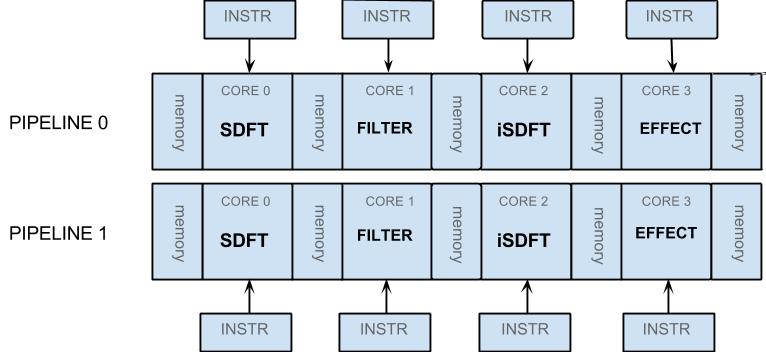
\includegraphics[height=150px]{figures/fpga/system_components_general_pipeline.png}
    \caption{Audio Pipeline Architecture}
    \label{fig:pipeline_architecture}
\end{figure}

\textit{ChaosM} consists of two audio processing pipelines, as illustrated in
Figure \ref{fig:pipeline_architecture}. These contain up to four processing cores
connected by data buffers. Each audio processing pipeline corresponds to one audio channel, operating on audio samples as elementary data elements.
The input/output frequency is directly tied to the sample rate of the input, which acts as a secondary clock input. The main system clock runs on the order of MHz, while this \textit{sample clk} is in the order of kHz and acts as a deadline for when new I/O is due.

\FloatBarrier
\section{Communication}

\subsection{The External Bus Interface}
The microcontroller communicates with the FPGA design using the External Bus
Interface (EBI) of the Giant Gecko microcontroller. The EBI is a parallel bus
with a separate data and address bus in addition to the chip select and read and
write enable signals, all active low\cite{efm_ebi}.

The communication between the MCU and the FPGA uses 23 address lines and 16
data lines. All transfers are initiated by the chip select signal going low.
Then, for write transfers, the data and address lines are set up and the
write enable signal is asserted, see figure \ref{fig:ebi_write}. For reads,
the address is set up and the data line is put in high impedance mode before
the read enable signal is asserted, see figure \ref{fig:ebi_read}.

\begin{figure}[h]
	\centering
	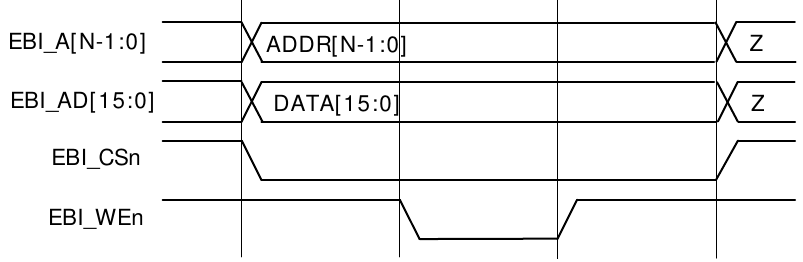
\includegraphics[width=0.8\linewidth]{figures/fpga/ebi_write.png}
	\caption{EBI write transfer\cite[p.6]{efm_ebi}}
	\label{fig:ebi_write}
\end{figure}



\begin{figure}[h]
	\centering
	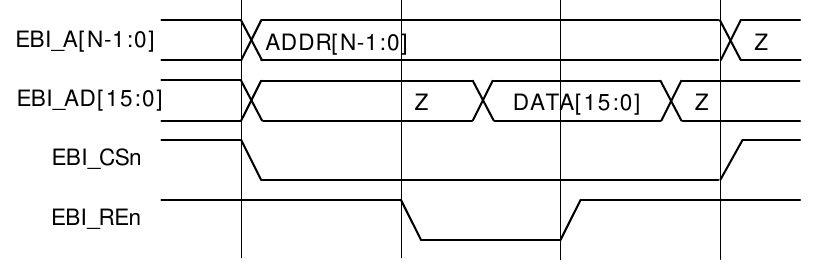
\includegraphics[width=0.8\linewidth]{figures/fpga/ebi_read.png}
	\caption{EBI read transfer\cite[p.7]{efm_ebi}}
	\label{fig:ebi_read}
\end{figure}



\FloatBarrier
\subsection{The Internal Bus}

The internal bus is used to transfer data to and from modules in the FPGA.
All transfers are initiated by the microcontroller on the EBI bus, and the
EBI controller module translates between the EBI and the internal bus.

\subsubsection{The EBI controller}
The EBI controller module is used to handle EBI transfers initiated by the
microcontroller. It consists of a simple state machine, illustrated in
figure \ref{fig:ebi_ctrl_fsm}. When an EBI transfer is executed, the
internal bus, described in is used to store or retrieve data from a module
in the FPGA.

In the idle state, the EBI data lines are set as high impedance, which
causes the microcontroller to have control of the data bus. Only when
a value is read over the EBI bus, does the EBI controller take control of
the data lines.

To save power, a clock gate is used to turn off the functional clock to
the EBI controller when the chip select signal is deasserted.

\begin{figure}[h]
	\centering
	% TODO: Make the arrows in separate directions be separate arrows
	\begin{tikzpicture}[shorten >= 1pt,node distance=2cm,on grid,auto]
		\node[state,initial] (idle) {idle};
		\node[state] (read) [above right=of idle] {read};
		\node[state] (write) [below right=of idle] {write};
		\path[->]
			(idle) edge node {\small RE = 0} (read)
			       edge node [swap] {\small EW = 0} (write)
			(read) edge node {\small RE = 1} (idle)
			(write) edge node [swap] {\small WE = 1} (idle);
	\end{tikzpicture}
	\caption{EBI controller state machine}
	\label{fig:ebi_ctrl_fsm}
\end{figure}




\subsubsection{Addressing}

Modules in the FPGA is addressed using a simple hierarchical scheme, where the
address is divided into three parts; the pipeline where the module is located,
the ``index'' of the module and an address specifying where in the module to
read or write data. Figure \ref{fig:ebi_addresses} illustrates the address
format.

\begin{figure}[H]
	\centering
	\begin{bytefield}[endianness=big,bitwidth=0.04\linewidth]{23}
		\bitheader{0-22}\\
		\bitbox{1}{T} &
		\bitbox{2}{\tiny Pipeline} &
		\bitbox{4}{Device} &
		\bitbox{2}{\tiny Subdev} &
		\bitbox{14}{Address}
	\end{bytefield}
	\caption{FPGA address format}
	\label{fig:ebi_addresses}
\end{figure}




\FloatBarrier
\subsubsection{Read Transfers}

A read transfer is initiated when the read enable line from the microcontroller goes low.
The EBI controller sets up the internal address signals and asserts the internal read enable
signal. This causes the requested data to be available in the next clock cycle. The EBI
controller switches to read state, where it remains until the read enable signal is deasserted.

\subsubsection{Write Transfers}

Write transfers are initiated the same way as read transfers. As the write-enable signal goes
low, the destination address is latched into the internal address bus and the internal data
lines are set to the value of the EBI data lines. The internal write enable signal is asserted
and the EBI controller enters the write state. In the write state the internal write enable
signal is reset, and when the EBI write enable signal is deasserted, idle mode is reentered.


% !TEX root = ../../../report.tex
\subsection{Instruction Set Architecture}\label{section:fpga-isa}

The processor was designed in a top-down fashion, starting with the instruction
set. The MIPS ISA used in the \textit{Computer
Design}\cite{tdt4255} course was a good starting point for the ISA used in this
project. In order to support as many different filters
and effects as possible, the processor supports all normal arithmetic
operations. Due to the requirements of doing Fourier transforms on the
processor, support for some floating point instructions was also included.

To make the decoding of instructions as easy as possible, instructions
were divided into three different instruction groups.

\subsubsection{Register-based Instructions}

The register-based instructions are instructions were both operands are
primarily registers. The group also includes a few instructions where
the second operand is an immediate value. The format of the
instructions are illustrated in Figure \ref{fig:regbased_instrs_format}. The
implemented functions can be found in Table \ref{tab:regbased_instrs}.

\begin{figure}[h]
	\centering
	\begin{bytefield}[bitwidth=0.05\linewidth]{16}
		\bitheader{0-15}	\\
		\bitbox{2}{Group}	&
		\bitbox{2}{Funct}	&
		\bitbox{2}{Opt}		&
		\bitbox{5}{Reg A}	&
		\bitbox{5}{Reg B/Imm}
	\end{bytefield}

	\caption{Register-based instruction format}
	\label{fig:regbased_instrs_format}
\end{figure}

\FloatBarrier
\begin{table}[H]
	\centering
	\begin{tabular}{|l l l l l|}
		\hline
		\textbf{Funct} & \textbf{Opt}  & \textbf{Mnemonic} & \textbf{Instruction} & \textbf{Operation} \\
	\hline
	\multicolumn{5}{|c|}{Group \texttt{0b00}} \\
	\hline
	\multirow{3}{*}{\texttt{0b00}}
		& \texttt{0b00} & \texttt{add \$ra, \$rb}  & Add registers & $\$ra \leftarrow \$ra + \$rb$ \\
		& \texttt{0b01} & \texttt{addi \$ra, imm} & Add immediate & $\$ra \leftarrow \$ra + imm$ \\
		& \texttt{0b10} & \texttt{fadd \$ra, \$rb} & Add registers (FP) & $\$ra \leftarrow \$ra + \$rb$ \\
	\multirow{4}{*}{\texttt{0b01}}
		& \texttt{0b00} & \texttt{sub \$ra, \$rb}  & Subtract registers & $\$ra \leftarrow \$ra - \$rb$ \\
		& \texttt{0b01} & \texttt{fsub \$ra, \$rb} & Subtract registers (FP) & $\$ra \leftarrow \$ra - \$rb$ \\
		& \texttt{0b10} & \texttt{cmp \$ra, \$rb}  & Compare & $cnd \leftarrow cnd(\$ra - \$rb)$ \\
		& \texttt{0b11} & - & compare fp / subtract imm? & - \\
	\multirow{4}{*}{\texttt{0b10}}
		& \texttt{0b00} & \texttt{mul \$ra, \$rb}  & Multiply registers & $\$ra \leftarrow \$ra * \$rb$ \\
		& \texttt{0b01} & \texttt{fmul \$ra, \$rb} & Multiply registers (FP) & $\$ra \leftarrow \$ra * \$rb$ \\
		& \texttt{0b10} & \texttt{fmla \$ra, \$rb} & Multiply-and-accumulate (FP) & $\$ra \leftarrow \$ra + \$rb * \$rc$ \\
		& \texttt{0b11} & \texttt{fmls \$ra, \$rb} & Multiply-and-subtract (FP) & $\$ra \leftarrow \$ra - \$rb * \$rc$ \\
	\multirow{2}{*}{\texttt{0b11}}
		& \texttt{0b00} & \texttt{shl \$ra, imm} & Shift left & $\$ra \leftarrow \$ra << imm$ \\
		& \texttt{0b01} & \texttt{shr \$ra, imm} & Shift right & $\$ra \leftarrow \$ra >> imm$\\
	\hline
	\multicolumn{5}{|c|}{Group \texttt{0b01}} \\
	\hline
	\multirow{2}{*}{\texttt{0b00}}
		& \texttt{0b00} & \texttt{and \$ra, \$rb} & And & $\$ra \leftarrow \$ra \wedge \$rb$ \\
		& \texttt{0b01} & \texttt{nand \$ra, \$rb} & Nand & $\$ra \leftarrow \neg(\$ra \wedge \$rb)$ \\
	\multirow{3}{*}{\texttt{0b01}}
		& \texttt{0b00} & \texttt{or \$ra, \$rb} & Or & $\$ra \leftarrow \$ra \vee \$rb$ \\
		& \texttt{0b01} & \texttt{nor \$ra, \$rb} & Nor & $\$ra \leftarrow \neg(\$ra \vee \$rb)$\\
		& \texttt{0b10} & \texttt{xor \$ra, \$rb} & Xor & $\$ra \leftarrow \$ra \oplus \$rb$\\
	\multirow{4}{*}{\texttt{0b10}}
		& \texttt{0b00} & \texttt{mov \$ra, \$rb} & Move & $\$ra \leftarrow \$rb$\\
		& \texttt{0b01} & \texttt{mvn \$ra, \$rb} & Move negative & $\$ra \leftarrow \neg\$rb$ \\
		& \texttt{0b10} & \texttt{i2f \$ra, \$rb} & Typecast (Int to FP) & $\$ra \leftarrow fp(\$rb)$ \\
		& \texttt{0b11} & \texttt{f2i \$ra, \$rb} & Typecast (Fp to int) & $\$ra \leftarrow int(\$rb)$ \\
	\multirow{4}{*}{\texttt{0b11}}
		& \texttt{0b00} & \texttt{lda \$ra, [\$rb]} & Load from input & $\$ra \leftarrow [\$rb]$ \\
		& \texttt{0b01} & \texttt{ldb \$ra, [\$rb]} & Load from output & $\$ra \leftarrow [\$rb]$ \\
		& \texttt{0b10} & \texttt{ldc \$ra, [\$rb]} & Load from constant buffer & $\$ra \leftarrow [\$rb]$ \\
		& \texttt{0b11} & \texttt{stb \$ra, [\$rb]} & Store to output & $[\$rb] \leftarrow \$ra$ \\
	\hline
	\end{tabular}
	\caption{Register-based instruction list}
	\label{tab:regbased_instrs}
\end{table}


\FloatBarrier

\subsubsection{Load Immediate Instruction}
The load immediate instruction is used to load an immediate constant into a
register. The format of the instruction can be found in figure
\ref{fig:ldi_format}. The value is loaded into register \texttt{\$r1}.

\begin{figure}[h]
	\centering
	\begin{bytefield}[bitwidth=0.05\linewidth]{16}
		\bitheader{0-15} \\
		\bitbox{2}{Group} &
		\bitbox{14}{Imm}
	\end{bytefield}

	\caption{Load immediate format}
	\label{fig:ldi_format}
\end{figure}

\FloatBarrier

\subsubsection{Branch Instruction}
The branch instruction checks condition flags and jumps accordingly. By
checking for various combinations of the condition flags, many different
conditions can be checked for. The format of the instruction is illustrated
in Figure \ref{fig:new_branch_format}.

\begin{figure}[h]
	\centering
	\begin{bytefield}[bitwidth=0.05\linewidth]{16}
		\bitheader{0-15} \\
		\bitbox{2}{Group} &
		\bitbox{4}{Flags} &
		\bitbox{11}{Target}
	\end{bytefield}

	\caption{Branch instruction format}
	\label{fig:new_branch_format}
\end{figure}


\FloatBarrier

\paragraph{Special Registers}

Due to the limited space in instruction words, only two registers at most can be
specified in an instruction. Some instructions, such as the load immediate and
load constant instructions do not specify any registers, only an immediate
offset constant.

The list of defined special registers can be found in Table \ref{tab:specregs}.

\begin{centering}[h]
	\begin{tabular}{|l p{10.5cm}|}
		\hline
		\textbf{Register name} & \textbf{Register purpose} \\
		\hline
		\texttt{r0} & Zero register, hard coded to always contain 0 \\
		\texttt{r1} & Immediate register, contains the result of an \textsc{ldi} instruction\\
		\texttt{rc} & Constant register, provides operand to \textsc{fmla} and \textsc{fmls} instructions. Lies within the ALU. \\
		\texttt{rc} & Constant register, provides operand to \textsc{fmla} and \textsc{fmls} instructions. Lies within the ALU. \\
		\hline
	\end{tabular}

	\label{tab:specregs}
	%\caption{List of special registers}
	
\end{centering}


\FloatBarrier

%!TEX root = ../../../report.tex

\subsection{Memory Types}\label{subsec:fpga-memory}

The internal block RAMs in the FPGA were used to implement the different kinds
of memories inside the processor. Even though this limits the amount of
memory available, it guarantees equal access time for all the different
of memories. It also precludes having to use external RAM, which would not be as
fast, nor energy-efficient.

All of the following memory types are implemented on the FPGA chip, and
therefore they all share the access time the block RAMs on the FPGA chip have.

\subsubsection{Instruction Memory}
Each processor core has a separate instruction memory. This memory is used to
store the program that is run by a processor core.

\subsubsection{Audio Pipeline Buffers}
The audio pipeline buffers are used for passing data through the audio pipeline.
Each core has an input buffer and an output buffer, which stores the samples
that are processesed by the core and the result respectively. The processors
have read-only access to their input buffers and read-write access to their
output buffers.

The buffers have two different modes of operation. In the switching mode,
the buffers are divided into two partitions. One partition is available
as output buffer for a core, and the other partition is available as the
input buffer for the next core. When the sample clock
changes, the buffer partitions are switched, thus passing data from the
output of one core to the input of the next.

When the ringbuffer mode is used, two sliding windows is used to partition
the buffer. Each core has access to their own window. On each sample clock
edge vthe window is advanced by a predefined number
of samples.

\subsubsection{Constant Memory}
The constant memory is used to store constants needed for computations. Each
audio pipeline contains one constant memory which is shared between two
configurable processors in the pipeline. This limitation is due to the block
RAM on the FPGA used, which has only two available read ports.


\FloatBarrier
\subsection{Processor Core}\label{subsec:fpga-processor-core}
\todo[inline]{How the processor is designed and why}

\subsubsection{Design Considerations}

The processor core is designed to be able to perform audio processing in real-time, and well as being as power efficient as possible. 
Since the FPGAs power usage is close to constant, the best way to save power is to reduce the time the whole board is active. 
The best way for the core to contribute to this is to execute its programs as fast as possible. Thus, the processor core has been designed by the two following principles:


\begin{itemize}
	\item As high throughput as possible.
	\item Support the instructions needed to perform the audio processing.
\end{itemize}

\subsubsection{Implementation}

In order for the core to be as efficient as possible, a pipelined processor
design was implemented. The pipelined core design consists of the following
stages:

\begin{enumerate}
	\item Instruction Fetch \label{stage:if}
	\item Instruction Decode \label{stage:id}
	\item Memory \label{stage:mem}
	\item Execute \label{stage:ex}
	\item Write back \label{stage:wb}
\end{enumerate}

A change from the classic pipelined processor designs, is that the memory stage comes before the execution stage. 
This is because the load and store instructions does not need the ALU to calculate the memory address. 
Thus the processor is able to prevent \textit{all} data dependecies by forwarding data from the different stages.

For simplicity, the core does not have a hazard control unit implemented for
branching. Instead it relies on the programmer to add two no-operations after a branch.




\FloatBarrier
\subsection{ALU}\label{subsection:fpga-alu}
\todo[inline]{ALU design and reasons why. -First revision finished?}

When the group sat down and started considering the ALU of our pipelined
processor cores, it was decided that we wanted to go for the ``Less is more''
design philosophy. This due to the fact that more often than not, the circuits
comprising the ALU logic tend to be the more resource-intensive and complicated
ones in a processor.

With that in mind, a following prioritization list of supported hardware
operations was made:\todo{This needs to be fleshed out when we've finished the
ALU.}
\begin{enumerate}
	\item Logic to allow for sufficiently fast Fourier-transforms (so that the
transform could be performed on each discrete sample within a single clockcycle
of the sequential processing core pipeline).
	\begin{enumerate}
		\item The Fourier-transform we settled on could be performed with only
addition, substraction, and shifting. Therefore hardware support for these
operations also had to be implemented.
	\end{enumerate}
	\item Multiplication for the sound-effect manipulations on the transformed
samples located in the frequency domain.
\end{enumerate}
\emph{For any reader potentially wondering, why division was left out, this is
explained in section \ref{subsubsection:fpga-alu-div}.}

\FloatBarrier
\subsubsection{Fourier-transforms}\label{subsubsection:fpga-alu-ft}
\todo[inline]{Need a way to refer to this subsubsection. I tried refering to it
in the design.tex file. The resulting reference refers to the ALU subsection as
a whole, and not the FT subsection.}

When it became necessary to start looking into how one implements a
Fourier-transform on a FPGA processor (as previously mentioned in section
\ref{section:fpga-design}), a lot of effort was spent on attemting to first find
examples of how others have implemented FT's (Fourier-transforms) on embedded
real-time devices before.

It did not take long before it became evident that there were two types of FT's
standing out from the rest of when considering FT's for the purpose of real-time
sound processing. Namely the Integer- and Sliding-Discrete- Fourier-Transforms.
The Integer-FT was ideal when considering that we would not have to implement
support for floating-point operations.

However, the Integer-FT needed the whole music file when transforming. It could
not transform discrete samples one at the time, which we would need if we had a
live source as input (say a portable music device connected to the PCB's
minijack). Also, we were unable to find any pseudo-code describing how such a
transform would function. The few examples we found described only the
mathematical functions, which left too huge a gap for us to research on our own.

Having found this out, the Sliding-Discrete-FTs potential use for our purposes
rose substantially. Not only would it allow us to perform a real-time
Fourier-transform, but we also managed to find pseudo-code describing how such a
transform would function. The big downside to the SD-FT however was the
necessity of floating-point to accomplish the implementation.

\FloatBarrier
\subsubsection{ALU input size}\todo{Better subsubsection title?}

Due to the algorithmically heavy operations of the SD-FT being the
\emph{heaviest} algorithmic operation performed in the the processor as a whole,
looking into how we could optimize the algorithm became a focus in the VHDL
group. Using the application \todo{Need references to actual (and correct!)
application notes here!}notes to find out the potential best speeds (read:
frequencies) of the FPGA, we then started calculating how fast the SD-FT would
have to perform its transform per sample.

It quickly became apparent that a ``quick and easy'' way to drastically reduce
the time complexity the algorithm would need to transform each sample, was to
reduce the sample sizes. \todo[inline]{Find some reference, or picture, or add a
paragraph explaining said algorithm.}With this in mind, we started testing how
small samples we could have, and yet have a passable level of sound quality. The
final result we ended up on was to have eight-bit datasamples. This had the
consequence of reducing the maximum sound frequency from ca. 44 kilohertz down
to \todo{This needs to be confirmed/edited.}11.

\FloatBarrier
\subsubsection{Leaving out division}\label{subsubsection:fpga-alu-div}

The decision to not implement hardware support for division was done for several
reasons. Firstly, hardware support for division is costly. Secondly, seeing as
we had already decided on having to implement floating-point for the SD-FT, we
decided that the amount of logic needed for each core to support both division
and floating-point was too much. Thirdly, having floating-point support, we
just as well multiply with a number smaller than one to perform a division. For
integer division it was decided that the programmer could program the cores to
perform longdivision with addition and substraction loop (or shifting when a
division by a power of 2 was attempted).


\subsection{Energy Efficiency}

\textit{ChaosM} is designed with a basic idea of energy efficiency. Since the
different cores in each pipeline perform different tasks, it is natural for them
to finish independently of each other. Therefore, \textit{ChaosM} is designed so
that it is possible to turn off the individual cores once they finish operating.
This functionality has a neglegible effect on the power consumption of an FPGA
and therefore doesn't affect energy efficiency on this particular system. If the
\textit{ChaosM} design was recreated as hardware on an integrated circuit,
however, this functionality could improve energy effieciency.

% !TEX root = ../../../report.tex

\subsection{Assembler}

Writing programs for a self-constructed ISA is cumbersome without utility
programs like compilers or assemblers. Thus, a simple assembler was written in
Haskell; the \textit{Hassembler}. It counts about 250 lines of code and uses the
monadic parser combinator library Parsec \cite{parsec}. The source code in its entirety is
released under a BSD3 licence available for download at
\url{https://github.com/terjr/hassembler}.

